\section{初等范畴论}

\subsection{范畴与函子}

\begin{definition}[范畴]
    \label {definition:category}
    一个范畴 \(\mathcal{C}\) 包含以下资料:

    \begin{enumerate}
        \item 一个类 \(\mathrm{Ob} (\mathcal{C})\), 称为对象类.
        \item 对于任意 \(\mathrm{Ob} (\mathcal{C})\) 中的对象 \(X,Y\), 分配态射集 \(\mathrm{Hom}_{\mathcal{C}} (A,B)\).
        \item 对任意对象 \(X\) 有单位映射 \(\mathrm{id}_X \in \mathrm{Hom}_{\mathcal{C}} (X,X)\).
        \item 对任意对象 \(X,Y,Z \in \mathcal{C}\) 有复合映射 \(\circ : \mathrm{Hom}_{\mathcal{C}} (Y,Z) \times \mathrm{Hom}_{\mathcal{C}} (X,Y) \to \mathrm{Hom}_{\mathcal{C}} (X,Z)\) 满足:
        \begin{enumerate}
            \item 结合律: \(\forall f \in \mathrm{Hom}_{\mathcal{C}} (Z,W), g \in \mathrm{Hom}_{\mathcal{C}} (Y,Z), h \in \mathrm{Hom}_{\mathcal{C}} (X,Y)\), 有 \((f \circ g) \circ h = f \circ (g \circ h)\).
            \item 单位元: \(\forall f \in \mathrm{Hom}_{\mathcal{C}} (X,Y)\), 有 \(f \circ \mathrm{id}_X = f = \mathrm{id}_Y \circ f\).
        \end{enumerate}
    \end{enumerate}
\end{definition}

\begin{definition}[交换图表]
    一个图表意味着由点代对象而由一个点至另一个点的箭头代表两对象间态射的, 比如:
    \begin{center}
        \begin{tikzpicture}
            \node (A) at (0,0) {\(A\)};
            \node (B) at (2,0) {\(B\)};
            \node (C) at (0,-2) {\(C\)};
            \node (D) at (2,-2) {\(D\)};
            \draw[->] (A) -- node[above] {\(f\)} (B);
            \draw[->] (A) -- node[left] {\(g\)} (C);
            \draw[->] (B) -- node[right] {\(h\)} (D);
            \draw[->] (C) -- node[below] {\(k\)} (D);
        \end{tikzpicture}
    \end{center}
    图表交换意味着两点间任意态射合成均相等, 比如 \(h \circ f = k \circ g\).
\end{definition}

\begin{example}
    定义 \(\mathbf{Set}\) 为集合范畴, 其中对象为集合, 对象间态射为映射.
\end{example}

\begin{example}
    定义 \(\mathbf{0}\) 为空范畴, 也即 \(\mathrm{Ob} (\mathbf{0}) = \emptyset\).
\end{example}

\begin{example}
    对偏序集 \(P\), 定义其对应的范畴 \(\mathrm{Cat} (P)\) 如下:

    \begin{enumerate}
        \item 对象是 \(P\) 中的元素.
        \item \(x \leq y\) 时有唯一态射 \(x \to y\).
        \item \(x \nleq y\) 时没有态射.
    \end{enumerate}
\end{example}

\begin{definition}
    对集合 \(S\) 定义离散范畴 \(\mathrm{Disc} (S)\) 如下:

    \begin{enumerate}
        \item 对象是 \(S\) 中的元素.
        \item 仅有单位态射.
    \end{enumerate}
\end{definition}

\begin{definition}
    若有一组映射 \(f : X \to Y\), \(g : Y \to X\) 使得 \(g \circ f = \mathrm{id}_X\), \(f \circ g = \mathrm{id}_Y\), 则称 \(f\) 为 \(g\) 的逆, \(f\) 是同构,
    记作 \(f^{-1} = g\).

    \(X\) 与 \(Y\) 同构记作 \(X \cong Y\), 命全体 \(X\) 与 \(Y\) 间的同构为 \(\mathrm{Isom}_{\mathcal{C}} (X,Y)\).
\end{definition}

\begin{definition}
    定义自同态集 \(\mathrm{End}_{\mathcal{C}} (X) := \mathrm{Hom}_{\mathcal{C}} (X,X)\) 与自同构集
    \(\mathrm{Aut}_{\mathcal{C}} (X) := \mathrm{Isom}_{\mathcal{C}} (X,X)\), 其上有自然的复合运算.
\end{definition}

\begin{definition}
    态射 \(f : X \to Y\) 称为单态射, 如果对于任意 \(g,h : Z \to X\), 有 \(f \circ g = f \circ h \implies g = h\).

    态射 \(f : X \to Y\) 称为满态射, 如果对于任意 \(g,h : Y \to Z\), 有 \(g \circ f = h \circ f \implies g = h\).
\end{definition}

\begin{definition}[反范畴]
    定义范畴 \(\mathcal{C}^{\mathrm{op}}\) 如下:

    \begin{enumerate}
        \item \(\mathrm{Ob} (\mathcal{C}^{\mathrm{op}}) = \mathrm{Ob} (\mathcal{C})\).
        \item \(\mathrm{Hom}_{\mathcal{C}^{\mathrm{op}}} (X,Y) = \mathrm{Hom}_{\mathcal{C}} (Y,X)\).
        \item 对于态射 \(f : X \to Y, g : Y \to Z\), 定义 \(g \circ_{\mathrm{op}} f := f \circ g\).
    \end{enumerate}
\end{definition}

\begin{definition}[函子]
    \label {definition:functor}
    一个函子 \(F : \mathcal{C} \to \mathcal{D}\) 包含以下资料:

    \begin{enumerate}
        \item 对象映射 \(F : \mathrm{Ob} (\mathcal{C}) \to \mathrm{Ob} (\mathcal{D})\).
        \item 对于任意对象 \(X,Y \in \mathcal{C}\), 有映射 \(F : \mathrm{Hom}_{\mathcal{C}} (X,Y) \to \mathrm{Hom}_{\mathcal{D}} (F(X),F(Y))\).
        \item 对于任意对象 \(X \in \mathcal{C}\), 映单位态射为单位态射 \(F(\mathrm{id}_X) = \mathrm{id}_{F(X)}\).
        \item 对于任意对象 \(X,Y,Z \in \mathcal{C}\) 保持态射的复合 \(F(g \circ f) = F(g) \circ F(f)\).
    \end{enumerate}
\end{definition}

\begin{definition}
    一个函子称为忠实 (faithful), 如果对于任意对象 \(X,Y \in \mathcal{C}\), 映射 \(F : \mathrm{Hom}_{\mathcal{C}} (X,Y) \to \mathrm{Hom}_{\mathcal{D}} (F(X),F(Y))\) 是单射.

    一个函子称为全 (full), 如果对于任意对象 \(X,Y \in \mathcal{C}\), 映射 \(F : \mathrm{Hom}_{\mathcal{C}} (X,Y) \to \mathrm{Hom}_{\mathcal{D}} (F(X),F(Y))\) 是满射.

    一个函子称本质满 (essentially surjective), 如果对于任意对象 \(Y \in \mathcal{D}\), 存在对象 \(X \in \mathcal{C}\) 使得 \(F(X) \cong Y\).
\end{definition}

\begin{definition}
    对于函子 \(F : \mathcal{C} \to \mathcal{D}\), \(G : \mathcal{D} \to \mathcal{E}\), 定义函子间的复合 \((G \circ F) (X) := G(F(X))\), \((G \circ F) (f) := G(F(f))\).

    \begin{proof}
        只需注意到 \(G(F(f)) \circ G(F(g)) = G(F(f) \circ F(g)) = G(F(f \circ g))\).
    \end{proof}
\end{definition}

\begin{definition}
    显见函子复合满足结合律, 定义范畴 \(\mathbf{Cat}\) 如下:

    \begin{enumerate}
        \item 对象是 \(\mathrm{Ob}\) 是集合的范畴.
        \item \(\mathrm{Hom}_{\mathbf{Cat}} (\mathcal{C},\mathcal{D})\) 是所有函子 \(\mathcal{C} \to \mathcal{D}\).
    \end{enumerate}
\end{definition}

\begin{definition}[自然变换]
    两个函子 \(F,G : \mathcal{C} \to \mathcal{D}\) 之间的自然变换 (natural transformation) \(\eta : F \to G\) 为对所有 \(X \in \mathrm{Ob} (C)\) 择定的态射 \(\eta_X : F(X) \to G(X)\),
    满足对于任意对象 \(X,Y \in \mathcal{C}\) 与 \(f \in \mathrm{Hom}_{\mathcal{C}} (X,Y)\), 有交换图表:
        
    \begin{center}
        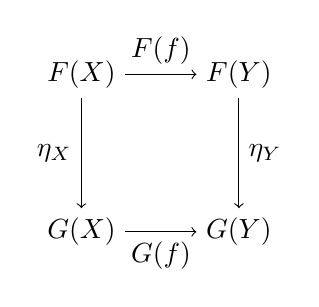
\begin{tikzpicture}
            \node (FX) at (0,0) {\(F(X)\)};
            \node (FY) at (2,0) {\(F(Y)\)};
            \node (GX) at (0,-2) {\(G(X)\)};
            \node (GY) at (2,-2) {\(G(Y)\)};
            \draw[->] (FX) -- node[above] {\(F(f)\)} (FY);
            \draw[->] (FX) -- node[left] {\(\eta_X\)} (GX);
            \draw[->] (FY) -- node[right] {\(\eta_Y\)} (GY);
            \draw[->] (GX) -- node[below] {\(G(f)\)} (GY);
        \end{tikzpicture}
    \end{center}

    记作 \(\eta : F \to G\), 可以画作图表:

    \begin{center}
        \begin{tikzpicture}
            \node (C) at (-2,0) {\(\mathcal{C}\)};
            \node (D) at (2,0) {\(\mathcal{D}\)};
            \draw[->] (C) to[bend left=60] node[above] (F) {\(F\)} (D);
            \draw[->] (C) to[bend right=60] node[below] (G) {\(G\)} (D);
            \draw[double,-{Implies},double distance = 0.15em] ($(F.south) + (0,- 0.1)$) to node[right] {\(\eta\)} ($(G.north) + (0,0.1)$);
        \end{tikzpicture}
    \end{center}
\end{definition}

\begin{definition}[纵合成]
    给出 \(\eta : F \to G\), \(\theta : G \to H\), 定义纵合成 \(\theta \circ \eta : F \to H\) 为 \({(\theta \circ \eta)}_X := \theta_X \circ \eta_X\), 解作图表:
    
    \begin{center}
        \begin{tikzpicture}
            \node (C) at (-2,0) {\(\mathcal{C}\)};
            \node (D) at (2,0) {\(\mathcal{D}\)};
            \draw[->] (C) to[bend left=60] node[above] (F) {\(F\)} (D);
            \draw[->] (C) to node[above] (G) {\(G\)} (D);
            \draw[->] (C) to[bend right=60] node[below] (H) {\(H\)} (D);
            \draw[double,-{Implies},double distance = 0.15em] ($(F.south) + (0,- 0.1)$) to node[right] {\(\eta\)} ($(G.north) + (0,0.1)$);
            \draw[double,-{Implies},double distance = 0.15em] ($(G.south) + (0,- 0.1)$) to node[right] {\(\theta\)} ($(H.north) + (0,0.1)$);
        \end{tikzpicture} \begin{tikzpicture}
            \node (C) at (-2,0) {\(\mathcal{C}\)};
            \node (D) at (2,0) {\(\mathcal{D}\)};
            \draw[->] (C) to[bend left=60] node[above] (F) {\(F\)} (D);
            \draw[->] (C) to[bend right=60] node[below] (H) {\(H\)} (D);
            \draw[double,-{Implies},double distance = 0.15em] ($(F.south) + (0,- 0.1)$) to node[right] {\(\theta \circ \eta\)} ($(H.north) + (0,0.1)$);
        \end{tikzpicture}
    \end{center}

    \begin{proof}
        只需注意到以下交换图表 (两小方块交换故外框交换):

        \begin{center}
            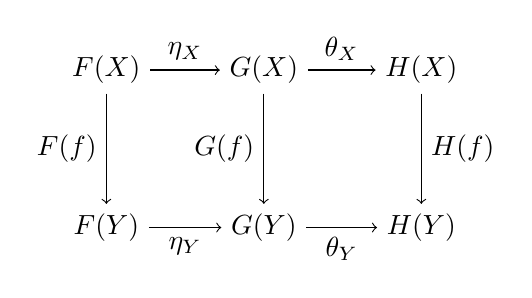
\begin{tikzpicture}
                \node (FX) at (-2,1) {\(F(X)\)};
                \node (FY) at (-2,-1) {\(F(Y)\)};
                \node (GX) at (0,1) {\(G(X)\)};
                \node (GY) at (0,-1) {\(G(Y)\)};
                \node (HX) at (2,1) {\(H(X)\)};
                \node (HY) at (2,-1) {\(H(Y)\)};
                \draw[->] (FX) -- node[left] {\(F(f)\)} (FY);
                \draw[->] (FX) -- node[above] {\(\eta_X\)} (GX);
                \draw[->] (FY) -- node[below] {\(\eta_Y\)} (GY);
                \draw[->] (GX) -- node[left] {\(G(f)\)} (GY);
                \draw[->] (GX) -- node[above] {\(\theta_X\)} (HX);
                \draw[->] (GY) -- node[below] {\(\theta_Y\)} (HY);
                \draw[->] (HX) -- node[right] {\(H(f)\)} (HY);
            \end{tikzpicture}
        \end{center}
    \end{proof}
\end{definition}

\begin{definition}[横合成]
    给出三个范畴 \(\mathcal{C},\mathcal{D},\mathcal{E}\) 以及四个函子 \(F_1,F_2 : \mathcal{C} \to \mathcal{D}\), \(G_1,G_2 : \mathcal{D} \to \mathcal{E}\), 给出自然变换 \(\eta : F_1 \to F_2\), \(\theta : G_1 \to G_2\), 定义横合成 \(\theta \ast \eta : G_1 \circ F_1 \to G_2 \circ F_2\) 为 \({(\theta \ast \eta)}_X := \theta_{F_2 (X)} \circ G_1 (\eta_X)\), 解作图表:

    \begin{center}
        \begin{tikzpicture}
            \node (C) at (-3,0) {\(\mathcal{C}\)};
            \node (D) at (0,0) {\(\mathcal{D}\)};
            \node (E) at (3,0) {\(\mathcal{E}\)};
            \draw[->] (C) to[bend left=40] node[above] (F1) {\(F_1\)} (D);
            \draw[->] (C) to[bend right=40] node[below] (F2) {\(F_2\)} (D);
            \draw[->] (D) to[bend left=40] node[above] (G1) {\(G_1\)} (E);
            \draw[->] (D) to[bend right=40] node[below] (G2) {\(G_2\)} (E);
            \draw[double,-{Implies},double distance = 0.15em] ($(F1.south) + (0,- 0.1)$) to node[right] {\(\eta\)} ($(F2.north) + (0,0.1)$);
            \draw[double,-{Implies},double distance = 0.15em] ($(G1.south) + (0,- 0.1)$) to node[right] {\(\theta\)} ($(G2.north) + (0,0.1)$);
        \end{tikzpicture} \begin{tikzpicture}
            \node (C) at (-2,0) {\(\mathcal{C}\)};
            \node (E) at (2,0) {\(\mathcal{E}\)};
            \draw[->] (C) to[bend left=40] node[above] (G1F1) {\(G_1 \circ F_1\)} (E);
            \draw[->] (C) to[bend right=40] node[below] (G2F2) {\(G_2 \circ F_2\)} (E);
            \draw[double,-{Implies},double distance = 0.15em] ($(G1F1.south) + (0,- 0.1)$) to node[right] {\(\theta \ast \eta\)} ($(G2F2.north) + (0,0.1)$);
        \end{tikzpicture}
    \end{center}

    \begin{proof}
        需注意到以下交换图表:

        \begin{center}
            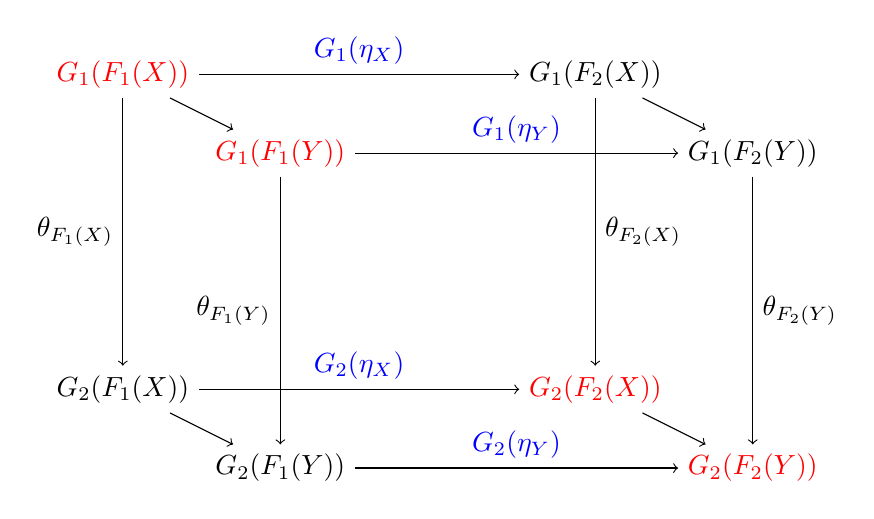
\begin{tikzpicture}
                \node (G1F1X) at (-4,4) {\textcolor{red}{\(G_1 (F_1 (X))\)}};
                \node (G1F1Y) at (-2,3) {\textcolor{red}{\(G_1 (F_1 (Y))\)}};
                \node (G1F2X) at (2,4) {\(G_1 (F_2 (X))\)};
                \node (G1F2Y) at (4,3) {\(G_1 (F_2 (Y))\)};
                \node (G2F1X) at (-4,0) {\(G_2 (F_1 (X))\)};
                \node (G2F1Y) at (-2,-1) {\(G_2 (F_1 (Y))\)};
                \node (G2F2X) at (2,0) {\textcolor{red}{\(G_2 (F_2 (X))\)}};
                \node (G2F2Y) at (4,-1) {\textcolor{red}{\(G_2 (F_2 (Y))\)}};
                \draw[->] (G1F1X) -- (G1F1Y);
                \draw[->] (G1F2X) -- (G1F2Y);
                \draw[->] (G2F1X) -- (G2F1Y);
                \draw[->] (G2F2X) -- (G2F2Y);
                \draw[->] (G1F1X) -- node[above] {\textcolor{blue}{\(G_1 (\eta_X)\)}} (G1F2X);
                \draw[->] (G1F1Y) -- node[above] {\textcolor{blue}{\(G_1 (\eta_Y)\)}} (G1F2Y);
                \draw[->] (G2F1X) -- node[above] {\textcolor{blue}{\(G_2 (\eta_X)\)}} (G2F2X);
                \draw[->] (G2F1Y) -- node[above] {\textcolor{blue}{\(G_2 (\eta_Y)\)}} (G2F2Y);
                \draw[->] (G1F1X) -- node[left] {{\(\theta_{F_1 (X)}\)}} (G2F1X);
                \draw[->] (G1F1Y) -- node[left] {\(\theta_{F_1 (Y)}\)} (G2F1Y);
                \draw[->] (G1F2X) -- node[right] {\(\theta_{F_2 (X)}\)} (G2F2X);
                \draw[->] (G1F2Y) -- node[right] {\(\theta_{F_2 (Y)}\)} (G2F2Y);
            \end{tikzpicture}
        \end{center}

        前后左右四面交换源自 \(\theta\) 为自然变换, 上下两面交换源自 \(\eta\) 为自然变换, 于是\textcolor{red}{红色}标记出的子图亦交换.
    \end{proof}
\end{definition}

特别的, 在标记自然变换时, 我们可以讲单独的函子 \(F\) 拉开成为 \(\mathrm{id}_F : F \to F\), 在每个 \(X\) 上为 \(\mathrm{id}_{F(X)}\).

\begin{definition}
    对于范畴 \(\mathcal{C}, \mathcal{D}\), 定义函子范畴 \(\mathbf{Fun} (\mathcal{C},\mathcal{D})\) 如下:

    \begin{enumerate}
        \item 对象是函子 \(\mathcal{C} \to \mathcal{D}\).
        \item 对于函子 \(F,G : \mathcal{C} \to \mathcal{D}\), 定义态射集 \(\mathrm{Hom}_{\mathbf{Fun} (\mathcal{C},\mathcal{D})} (F,G)\) 为所有 \(F \to G\) 的自然变换.
        \item 态射的合成是自然变换的纵合成.
    \end{enumerate}

    \begin{proof}
        只需证明纵合成之结合律, 只需注意到态射结合律:

        \[
            (\theta_X \circ \eta_X) \circ \phi_X = \theta_X \circ (\eta_X \circ \phi_X)
        \]
    \end{proof}
\end{definition}

\begin{lemma}
    函子的纵合成满足结合律.

    \begin{proof}
        给出自然变换 \(\theta, \psi, \phi\) 如下:

        \begin{center}
            \begin{tikzpicture}
                \node (C) at (-3,0) {\(\mathcal{C}\)};
                \node (D) at (-1,0) {\(\mathcal{D}\)};
                \node (E) at (1,0) {\(\mathcal{E}\)};
                \node (F) at (3,0) {\(\mathcal{F}\)};
                \draw[->] (C) to[bend left=40] node[above] (F1) {\(F_1\)} (D);
                \draw[->] (C) to[bend right=40] node[below] (F2) {\(F_2\)} (D);
                \draw[->] (D) to[bend left=40] node[above] (G1) {\(G_1\)} (E);
                \draw[->] (D) to[bend right=40] node[below] (G2) {\(G_2\)} (E);
                \draw[->] (E) to[bend left=40] node[above] (H1) {\(H_1\)} (F);
                \draw[->] (E) to[bend right=40] node[below] (H2) {\(H_2\)} (F);
                \draw[double,-{Implies},double distance = 0.15em] ($(F1.south) + (0,- 0.1)$) to node[right] {\(\eta\)} ($(F2.north) + (0,0.1)$);
                \draw[double,-{Implies},double distance = 0.15em] ($(G1.south) + (0,- 0.1)$) to node[right] {\(\theta\)} ($(G2.north) + (0,0.1)$);
                \draw[double,-{Implies},double distance = 0.15em] ($(H1.south) + (0,- 0.1)$) to node[right] {\(\psi\)} ($(H2.north) + (0,0.1)$);
            \end{tikzpicture}
        \end{center}

        有交换图表 (交换性源自于施 \(\psi\) 自然性于 \(G_2 \eta_X\)):

        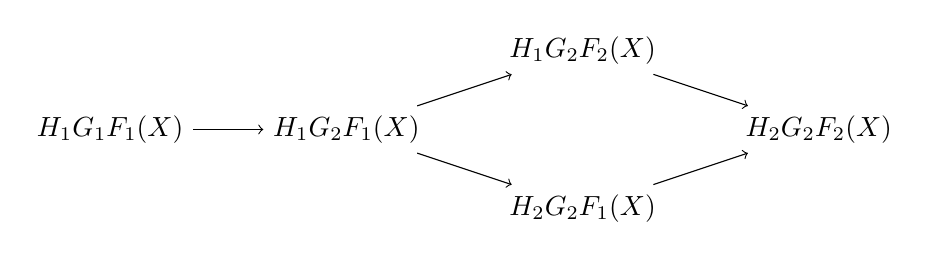
\begin{tikzpicture}
            \node (H1G1F1) at (-4.5,0) {\(H_1 G_1 F_1 (X)\)};
            \node (H1G2F1) at (-1.5,0) {\(H_1 G_2 F_1 (X)\)};
            \node (H1G2F2) at (1.5,1) {\(H_1 G_2 F_2 (X)\)};
            \node (H2G2F2) at (4.5,0) {\(H_2 G_2 F_2 (X)\)};
            \node (H2G2F1) at (1.5,-1) {\(H_2 G_2 F_1 (X)\)};
            \draw[->] (H1G1F1) -- (H1G2F1);
            \draw[->] (H1G2F1) -- (H1G2F2);
            \draw[->] (H1G2F2) -- (H2G2F2);
            \draw[->] (H1G2F1) -- (H2G2F1);
            \draw[->] (H2G2F1) -- (H2G2F2);
        \end{tikzpicture}
    \end{proof}
\end{lemma}

\begin{lemma}
    函子的横纵合成交换, 即亦给出自然变换如下:

    \begin{center}
        \begin{tikzpicture}
            \node (C) at (-3,0) {\(\mathcal{C}\)};
            \node (D) at (0,0) {\(\mathcal{D}\)};
            \node (E) at (3,0) {\(\mathcal{E}\)};
            \draw[->] (C) to[bend left=60] node[above] (F1) {\(F_1\)} (D);
            \draw[->] (C) to node[below] (F2) {\(F_2\)} (D);
            \draw[->] (C) to[bend right=60] node[below] (F3) {\(F_3\)} (D);
            \draw[->] (D) to[bend left=60] node[above] (G1) {\(G_1\)} (E);
            \draw[->] (D) to node[below] (G2) {\(G_2\)} (E);
            \draw[->] (D) to[bend right=60] node[below] (G3) {\(G_3\)} (E);
            \draw[double,-{Implies},double distance = 0.15em] ($(F1.south) + (0,- 0.1)$) to node[right] {\(\eta\)} ($(F2.north) + (0,0.1)$);
            \draw[double,-{Implies},double distance = 0.15em] ($(F2.south)$) to node[right] {\(\eta^\prime\)} ($(F3.north) + (0,0.1)$);
            \draw[double,-{Implies},double distance = 0.15em] ($(G1.south) + (0,- 0.1)$) to node[right] {\(\theta\)} ($(G2.north) + (0,0.1)$);
            \draw[double,-{Implies},double distance = 0.15em] ($(G2.south)$) to node[right] {\(\theta^\prime\)} ($(G3.north) + (0,0.1)$);
        \end{tikzpicture}
    \end{center}

    则有等式 \((\theta^\prime \ast \eta^\prime) \circ (\theta \ast \eta) = (\theta^\prime \circ \theta) \ast (\eta^\prime \circ \eta)\).

    \begin{proof}
        只需注意到以下交换图表:

        \begin{center}
            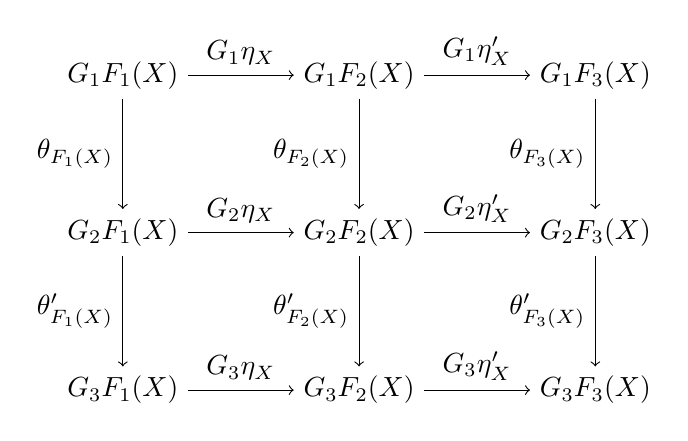
\begin{tikzpicture}
                \node (G1F1X) at (-3,2) {\(G_1 F_1 (X)\)};
                \node (G1F2X) at (0,2) {\(G_1 F_2 (X)\)};
                \node (G1F3X) at (3,2) {\(G_1 F_3 (X)\)};
                \node (G2F1X) at (-3,0) {\(G_2 F_1 (X)\)};
                \node (G2F2X) at (0,0) {\(G_2 F_2 (X)\)};
                \node (G2F3X) at (3,0) {\(G_2 F_3 (X)\)};
                \node (G3F1X) at (-3,-2) {\(G_3 F_1 (X)\)};
                \node (G3F2X) at (0,-2) {\(G_3 F_2 (X)\)};
                \node (G3F3X) at (3,-2) {\(G_3 F_3 (X)\)};
                \draw[->] (G1F1X) to node[above] {\(G_1 \eta_X\)} (G1F2X);
                \draw[->] (G1F2X) to node[above] {\(G_1 \eta^\prime_X\)} (G1F3X);
                \draw[->] (G2F1X) to node[above] {\(G_2 \eta_X\)} (G2F2X);
                \draw[->] (G2F2X) to node[above] {\(G_2 \eta^\prime_X\)} (G2F3X);
                \draw[->] (G3F1X) to node[above] {\(G_3 \eta_X\)} (G3F2X);
                \draw[->] (G3F2X) to node[above] {\(G_3 \eta^\prime_X\)} (G3F3X);
                \draw[->] (G1F1X) to node[left] {\(\theta_{F_1 (X)}\)} (G2F1X);
                \draw[->] (G1F2X) to node[left] {\(\theta_{F_2 (X)}\)} (G2F2X);
                \draw[->] (G1F3X) to node[left] {\(\theta_{F_3 (X)}\)} (G2F3X);
                \draw[->] (G2F1X) to node[left] {\(\theta^\prime_{F_1 (X)}\)} (G3F1X);
                \draw[->] (G2F2X) to node[left] {\(\theta^\prime_{F_2 (X)}\)} (G3F2X);
                \draw[->] (G2F3X) to node[left] {\(\theta^\prime_{F_3 (X)}\)} (G3F3X);
            \end{tikzpicture}
        \end{center}

        每个小正方形交换源于 \(\theta, \theta^\prime\) 为自然变换, 故外框交换.
    \end{proof}
\end{lemma}

\begin{lemma}
    自然变换 \(\eta : F \to G\) 是同构当且仅当对于任意 \(X \in \mathcal{C}\), \(\eta_X\) 是同构,
    其逆为 \(\eta^{-1} : G \to F\), \(\eta^{-1}_X := {\eta_X}^{-1}\).

    \begin{proof}
        给出其逆业已给出每个 \(\eta_X\) 之逆, 而 \(\eta^{-1}\) 是自然性对应了
        \(\eta\) 自然性的交换图表, 换言之, 以下图表每一小块交换故外框交换.

        \begin{center}
            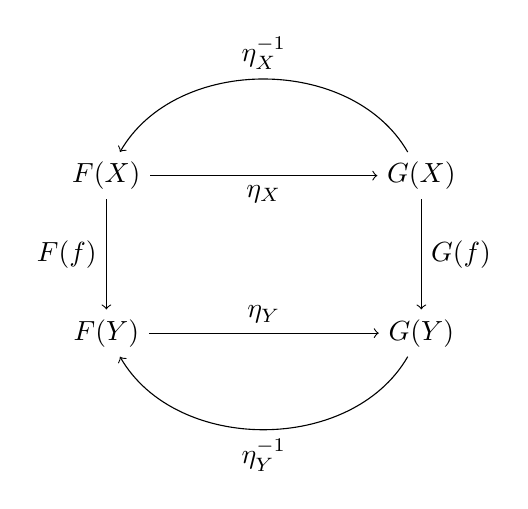
\begin{tikzpicture}
                \node (FX) at (-2,1) {\(F(X)\)};
                \node (FY) at (-2,-1) {\(F(Y)\)};
                \node (GX) at (2,1) {\(G(X)\)};
                \node (GY) at (2,-1) {\(G(Y)\)};
                \draw[->] (FX) to node[left] {\(F(f)\)} (FY);
                \draw[->] (FX) to node[below] {\(\eta_X\)} (GX);
                \draw[->] (FY) to node[above] {\(\eta_Y\)} (GY);
                \draw[->] (GX) to node[right] {\(G(f)\)} (GY);
                \draw[->] (GX) to [bend right=60] node[above] {\(\eta^{-1}_X\)} (FX);
                \draw[->] (GY) to [bend left=60] node[below] {\(\eta^{-1}_Y\)} (FY);
            \end{tikzpicture}
        \end{center}
    \end{proof}
\end{lemma}

\begin{definition}[范畴等价]
    若存在函子 \(F : \mathcal{C} \to \mathcal{D}\), \(G : \mathcal{D} \to \mathcal{C}\) 使得 \(G \circ F \cong \mathrm{id}_{\mathcal{C}}\), \(F \circ G \cong \mathrm{id}_{\mathcal{D}}\), 则称 \(\mathcal{C}\) 与 \(\mathcal{D}\) 等价.

    假定上述定义中 \(\cong\) 为 \(=\), 则称 \(\mathcal{C}\) 与 \(\mathcal{D}\) 同构.
\end{definition}

\begin{definition}[子范畴]
    给定范畴 \(\mathcal{C}^\prime, \mathcal{C}\), 若 \(\mathrm{Ob} (\mathcal{C}^\prime) \subseteq \mathrm{Ob} (\mathcal{C})\), 
    \(\mathrm{Hom}_{\mathcal{C}^\prime} (X,Y) \subseteq \mathrm{Hom}_{\mathcal{C}} (X,Y)\), 且保持复合运算,
    则称 \(\mathcal{C}^\prime\) 是 \(\mathcal{C}\) 的子范畴 (subcategory), 子范畴对应一个自然的嵌入 \(\iota : \mathcal{C}^\prime \to \mathcal{C}\),
    总是忠实, 子范畴亦有全和本质满的性质.
\end{definition}

\begin{definition}[骨架]
    如果范畴 \(\mathcal{C}^\prime\) 是 \(\mathcal{C}\) 的全子范畴, 且对于任意 \(X \in \mathrm{Ob} (\mathcal{C})\),
    都存在唯一 \(X^\prime \in \mathrm{Ob} (\mathcal{C}^\prime)\) 使得 \(X \cong X^\prime\), 则称 \(\mathcal{C}^\prime\) 是 \(\mathcal{C}\) 的骨架 (skeleton).

    自身是骨架的范畴称为骨架范畴 (skeletal category).
\end{definition}

\begin{definition}[小范畴]
    为了避免一些集合论的困难, 我们定义小范畴 (small category) 为对象类是集合的范畴.

    给出一个 Grothendieck 宇宙 \(\mathcal{U}\), 定义 \(\mathcal{U}\)-小范畴为对象类是 \(\mathcal{U}\) 中的集合的范畴.
\end{definition}

\begin{lemma}
    任何小范畴 \(\mathcal{C}\) 有骨架, 且骨架范畴与 \(\mathcal{C}\) 等价.

    \begin{proof}
        注意到 \(\cong\) 显见的是 \(\mathrm{Ob} (\mathcal{C})\) 上的等价关系, 在每个等价类
        上使用 \ref{axiom:NBG Axiom of Choice} 选取代表元 \(X^\prime\), 与等价类中任意一 \(X\) 与 \(X^\prime\) 间同构 \(f_X : X \to X^\prime\),
        选取子范畴 \(\mathcal{C}^\prime\) 如下:

        \begin{enumerate}
            \item 对象集为全体代表元 \(X^\prime\).
            \item 对于任意 \(X^\prime,Y^\prime \in \mathrm{Ob} (\mathcal{C}^\prime)\), \(\mathrm{Hom}_{\mathcal{C}^\prime} (X^\prime,Y^\prime) = \mathrm{Hom}_{\mathcal{C}} (X^\prime,Y^\prime) \).
        \end{enumerate}

        定义 \(\iota^{-1}\) 映 \(X\) 为其代表元 \(X^\prime\), 映 \(f \in \mathrm{Hom}_{\mathcal{C}} (X,Y)\) 为 
        \(f_Y \circ f \circ {f_X}^{-1}\).

        \(\iota^{-1}\) 函子性, \(\iota \circ \iota^{-1} = \mathrm{id}_{\mathcal{C}}\) 是显然的, 而构造 \(\iota^{-1} \circ \iota \cong \mathrm{id}_{\mathcal{C}^\prime}\) 的自然变换为 \(f\) 即可.
    \end{proof}
\end{lemma}

\begin{lemma}
    范畴等价具有传递性.

    \begin{proof}
        给出范畴 \(\mathcal{C},\mathcal{D},\mathcal{E}\), 函子 \(F : \mathcal{C} \to \mathcal{D}\), \(G : \mathcal{D} \to \mathcal{E}\), 
        以及其逆, 给出可逆的自然变换 \(\eta : F \circ F^{-1} \to \mathrm{id}_{\mathcal{D}}\), \(\theta : F^{-1} \circ F \to \mathrm{id}_{\mathcal{C}}\),
        \(\eta^\prime : G \circ G^{-1} \to \mathrm{id}_{\mathcal{E}}\), \(\theta^\prime : G^{-1} \circ G \to \mathrm{id}_{\mathcal{D}}\), 构造自然变换
        \(\eta^\prime \circ (\mathrm{id}_G \ast \eta \ast \mathrm{id}_{G^{-1}}) : G \circ F \circ F^{-1} \circ G^{-1} \to \mathrm{id}_{\mathcal{E}}\) 有逆
        \((\mathrm{id}_G \ast \eta^{-1} \ast \mathrm{id}_{G^{-1}}) \circ {\eta^{\prime}}^{-1}\),  \(\theta\) 侧可同理构造.
    \end{proof}
\end{lemma}

\begin{lemma}
    骨架范畴间的全忠实本质满函子都是同构.

    \begin{proof}
        本质满则在对象集上是双射, 全忠实亦给出每个态射集上的双射.
    \end{proof}
\end{lemma}

\begin{lemma}
    小范畴间函子 \(F\) 是等价当且仅当 \(F\) 全忠实本质满.

    \begin{proof}
        易得骨架范畴间的同构, 考虑等价的传递性即可.
    \end{proof}
\end{lemma}

\subsection{Hom 函子与泛性质}

\begin{definition}
    对于集合 \(I\) 与小范畴 \({(\mathcal{C}_i)}_{i \in I}\), 定义积范畴 \(\prod_{i \in I} \mathcal{C}_i\) 如下:

    \begin{enumerate}
        \item 对象是积 \(\prod_{i \in I} \mathrm{Ob} (\mathcal{C}_i)\) 的元素.
        \item 对于对象 \((X_i)_{i \in I}\), \((Y_i)_{i \in I}\), 定义态射集 \(\mathrm{Hom}_{\prod_{i \in I} \mathcal{C}_i} ((X_i)_{i \in I},(Y_i)_{i \in I})\) 为态射集之积
                \(\prod_{i \in I} \mathrm{Hom}_{\mathcal{C}_i} (X_i,Y_i)\).
        \item 态射的合成是逐点的, 也即 \({(f_i)}_{i \in I} \circ {(g_i)}_{i \in I} = {(f_i \circ g_i)}_{i \in I}\).
    \end{enumerate}

    定义余积范畴 \(\coprod_{i \in I} \mathcal{C}_i\) 如下:

    \begin{enumerate}
        \item 对象是无交并 \(\coprod_{i \in I} \mathrm{Ob} (\mathcal{C}_i)\) 的元素.
        \item 对象 \(X,Y\) 间有态射当且仅当其对应同一个 \(\mathcal{C}_i\), 态射集继承自 \(\mathcal{C}_i\).
    \end{enumerate}

    定义自明的投影函子 \(\mathbf{Pr}_j : \prod_{i \in I} \mathcal{C}_i \to \mathcal{C}_j\) 与包含函子 \(\mathbf{In}_j : \mathcal{C}_j \to \coprod_{i \in I} \mathcal{C}_i\).
\end{definition}

\begin{definition}
    多元函子即为从积范畴出发的函子.
\end{definition}

\begin{definition}[Hom 函子]
    对于任意范畴 \(\mathcal{C}\), 有函子 \(\mathrm{Hom}_{\mathcal{C}} (-,-) : \mathcal{C}^{\mathrm{op}} \times \mathcal{C} \to \mathbf{Set}\), 映 \((X,Y)\) 为态射集 \(\mathrm{Hom}_{\mathcal{C}} (X,Y)\), 
    映 \(\mathcal{C}^{\mathrm{op}} \times \mathcal{C}\) 中态射 \((f,g)\) 为映射 \(\phi \mapsto g \circ \phi \circ f\).

    称 \(\phi\) 对 \(f\) 做拉回 (pullback), 对 \(g\) 做推出 (pushforward).
\end{definition}
